\documentclass[tikz,border=2pt]{standalone}
\usepackage{amsmath,amssymb}
\usepackage{tikz}
\usetikzlibrary{arrows.meta}

\begin{document}
% A continuous f on a compact set X (here a closed disc, f = x1 + x2/2 with parallel level
% lines) attains a maximum M and a minimum m; its image is the compact interval [m, M].
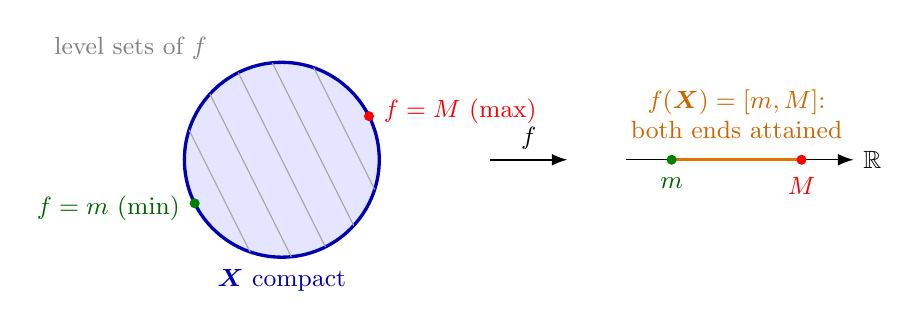
\begin{tikzpicture}[scale=0.825,  every node/.style={font=\small}, >={Latex[length=2mm]}]
	\fill[blue!10] (0,0) circle (1.5);
	\draw[blue!70!black, very thick] (0,0) circle (1.5);
	\begin{scope}
		\clip (0,0) circle (1.5);
		\foreach \c in {-1.2,-0.6,0,0.6,1.2} {
			\draw[gray!70, thin] ({\c-1.5},3) -- ({\c+1.5},-3);
		}
	\end{scope}
	\node[gray, font=\small, anchor=south east] at (-1.0,1.4) {level sets of $f$};
	\fill[red] (1.342,0.671) circle (2.2pt);
	\node[red, right] at (1.42,0.75) {$f=M$ (max)};
	\fill[green!50!black] (-1.342,-0.671) circle (2.2pt);
	\node[green!40!black, left] at (-1.42,-0.75) {$f=m$ (min)};
	\node[blue!70!black] at (0,-1.85) {$\boldsymbol{X}$ compact};
	\draw[->, thick] (3.2,0) -- (4.4,0) node[midway, above] {$f$};
	\begin{scope}[xshift=5.6cm]
		\draw[-{Latex[length=2mm]}] (-0.3,0) -- (3.2,0) node[right] {$\mathbb{R}$};
		\draw[very thick, orange!90!black] (0.4,0) -- (2.4,0);
		\fill[green!50!black] (0.4,0) circle (2.2pt);
		\fill[red] (2.4,0) circle (2.2pt);
		\node[below=3pt, green!40!black] at (0.4,0) {$m$};
		\node[below=3pt, red] at (2.4,0) {$M$};
		\node[orange!80!black, above=4pt, align=center] at (1.4,0) {$f(\boldsymbol{X})=[m,M]$:\\ both ends attained};
	\end{scope}
\end{tikzpicture}
\end{document}
